%%%%%%%%%%%%%%%%%%%%%%%%%%%%%%%%%%%%%%%%%%%%%%%%%%%%%%%%%%%%%%%%%%%%%%
% Problem statement
\begin{statement}[
  problempoints=100,
  timelimit=3 sekunde,
  memorylimit=512 MiB,
]{Standardni}

Ovo je priča o dvojici kolega, Stjepanu i Ljubi, koji od dosade ne znaju što bi
sami sa sobom pa su odlučili proučavati origami, tradicionalnu japansku
tehniku presavijanja papira. U te im je svrhe trebalo više papira raznih
dimenzija, a Ljubo je u džepu pronašao samo jedan papir dimenzija $A\times B$.
Srećom, Stjepan je ponio škare i naši su se junaci bacili na posao.

Stjepan je ukupno napravio $N$ horizontalnih (duž stranice duljine $A$) i
vertikalih (duž stranice duljine $B$) rezova. Nakon svakog su reza nastali
neki novi, manji komadi papira.  Provjere radi, Ljubo je nakon svakog
Stjepanovog reza zapisao najveću površinu nekog od dobivenih komada papira.

Ako su vam poznate početne dimenzije papira, kao i svaki Stjepanov rez, možete
li odrediti koje je brojeve Ljubo zapisao?

%%%%%%%%%%%%%%%%%%%%%%%%%%%%%%%%%%%%%%%%%%%%%%%%%%%%%%%%%%%%%%%%%%%%%%
% Input
\subsection*{Ulazni podaci}
U prvom su retku prirodni brojevi $A$, $B$ i $N$ $(1 \le N \le A + B - 2)$ iz
teksta zadatka.

Svaki od sljedećih $N$ redaka predstavlja jedan Stjepanov rez. Svaki je redak
oblika ``\texttt{H y}'' ili ``\texttt{V x}''. U prvom se slučaju radi o
horizontalnom rezu za $y$ $(1 \le y < B)$ udaljenom od donjeg ruba papira, dok
se u drugom slučaju radi o vertikalnom rezu za $x$ $(1 \le x < A)$ udaljenom
od lijevog ruba papira.

Stjepan nikada neće napraviti dva ista reza.

%%%%%%%%%%%%%%%%%%%%%%%%%%%%%%%%%%%%%%%%%%%%%%%%%%%%%%%%%%%%%%%%%%%%%%
% Output
\subsection*{Izlazni podaci}
U $i$-tom od $N$ redaka ispišite najveću površinu nekog komada papira nakon
$i$-tog Stjepanovog reza.

%%%%%%%%%%%%%%%%%%%%%%%%%%%%%%%%%%%%%%%%%%%%%%%%%%%%%%%%%%%%%%%%%%%%%%
% Scoring
\subsection*{Bodovanje}
{\renewcommand{\arraystretch}{1.4}
  \setlength{\tabcolsep}{6pt}
  \begin{tabular}{ccl}
 Podzadatak & Broj bodova & Ograničenja \\ \midrule
  1 & 20 & $2 \le A, B \le 500\,000$, $N = 1$\\
  2 & 20 & $2 \le A, B \le 100$ \\
  3 & 20 & $A = 1$, $2 \le B \le 500\,000$ \\
  4 & 20 & $2 \le A, B \le 1\,000$ \\
  5 & 20 & $2 \le A, B \le 500\,000$ \\
\end{tabular}}

%%%%%%%%%%%%%%%%%%%%%%%%%%%%%%%%%%%%%%%%%%%%%%%%%%%%%%%%%%%%%%%%%%%%%%
% Examples
\subsection*{Probni primjeri}
\begin{tabularx}{\textwidth}{X'X'X}
\sampleinputs{test/standardni.dummy.in.1}{test/standardni.dummy.out.1} &
\sampleinputs{test/standardni.dummy.in.2}{test/standardni.dummy.out.2} &
\sampleinputs{test/standardni.dummy.in.3}{test/standardni.dummy.out.3}
\end{tabularx}

\textbf{Pojašnjenje drugog probnog primjera:}
\begin{figure}[H]
\centering
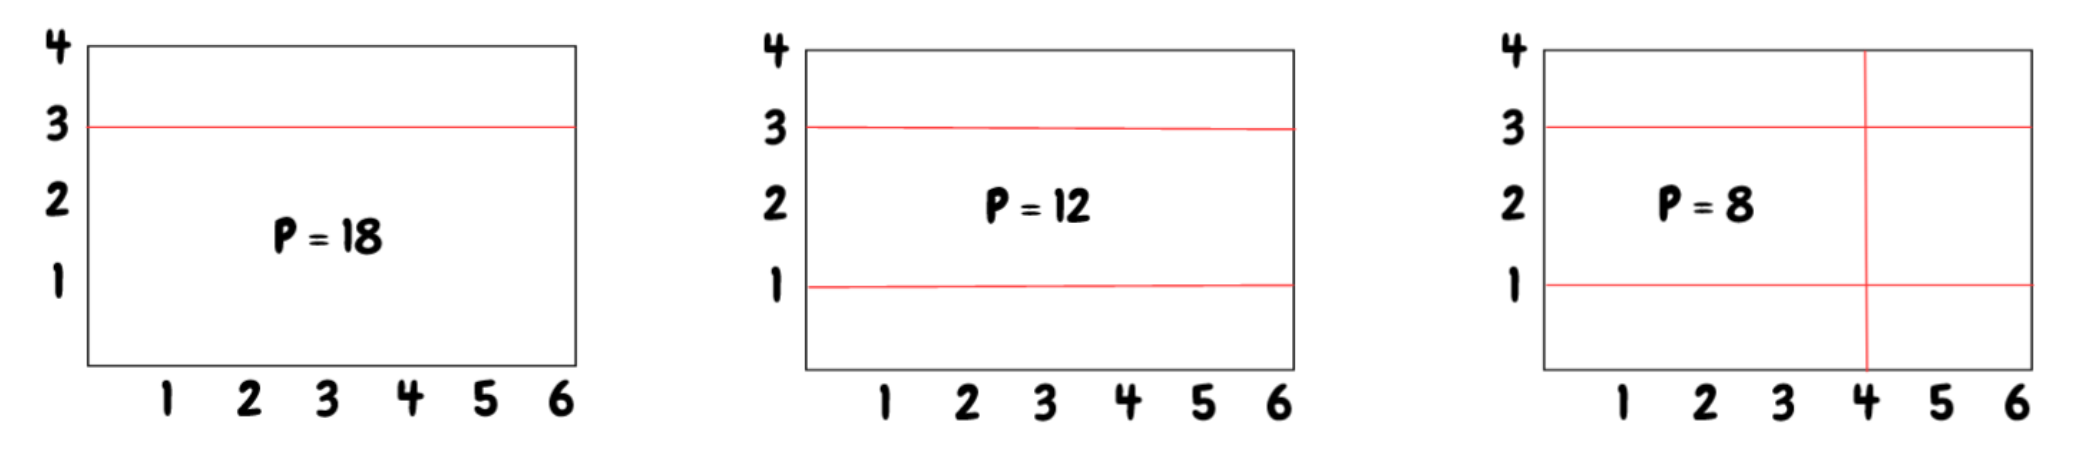
\includegraphics[width=\textwidth]{img/standardni_skica.png}
\end{figure}

%%%%%%%%%%%%%%%%%%%%%%%%%%%%%%%%%%%%%%%%%%%%%%%%%%%%%%%%%%%%%%%%%%%%%%
% We're done
\end{statement}

%%% Local Variables:
%%% mode: latex
%%% mode: flyspell
%%% ispell-local-dictionary: "croatian"
%%% TeX-master: "../hio.tex"
%%% End:
